% !TEX program = xelatex
% 在 Overleaf 中选择 XeLaTeX；编辑本文件即可。
\documentclass{resume}
\usepackage[UTF8,scheme=plain,fontset=fandol]{ctex}
% Compact two-column header shared by Chinese and English documents.
\usepackage{graphicx}
% Upload photo.jpg or photo.png to the same directory as main.tex.
% Photos are scaled proportionally to fit within 2.8 cm x 3.7 cm.
\newcommand{\cvphotobox}{%
  \IfFileExists{photo.jpg}{%
    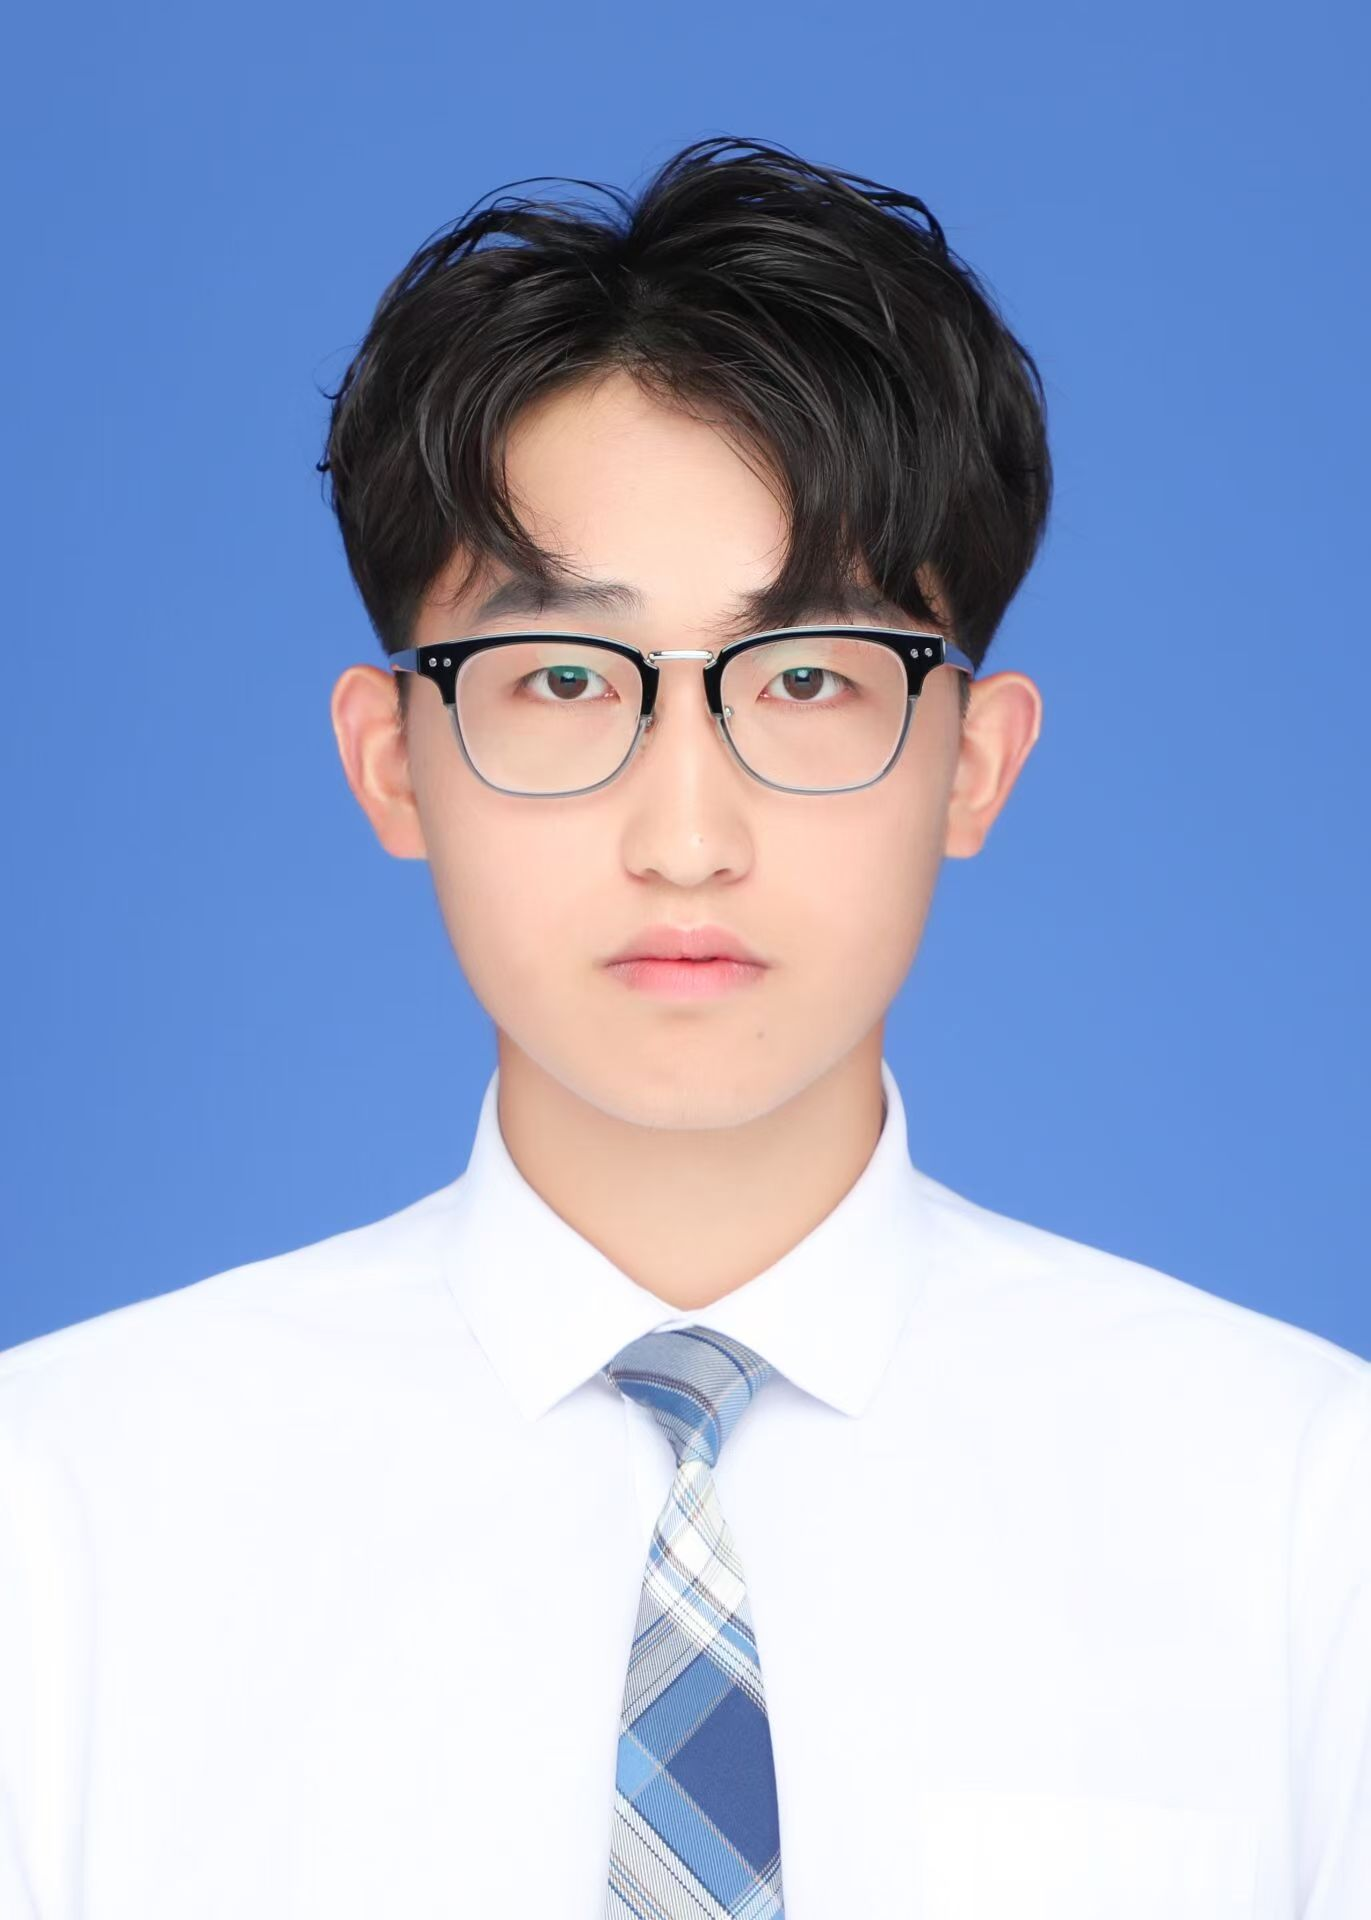
\includegraphics[width=2.8cm,height=3.7cm,keepaspectratio]{photo.jpg}%
  }{%
    \IfFileExists{photo.png}{%
      \includegraphics[width=2.8cm,height=3.7cm,keepaspectratio]{photo.png}%
    }{%
      {\setlength{\fboxsep}{0pt}\setlength{\fboxrule}{0.3pt}\color{accent!25}%
      \fbox{\parbox[c][3.7cm][c]{2.8cm}{\centering
        \normalfont\scriptsize\color{accent!65}PHOTO\\[3pt]
        photo.jpg / photo.png}}}%
    }%
  }%
}
\newcommand{\cvheader}[2]{%
  \noindent
  \begin{minipage}[c]{\dimexpr\textwidth-3.3cm\relax}
    \raggedright
    {\fontsize{27pt}{32pt}\selectfont\bfseries #1\par}
    \vspace{4pt}
    {\fontsize{11pt}{14.5pt}\selectfont #2\par}
  \end{minipage}\hfill
  \begin{minipage}[c]{2.8cm}
    \centering\cvphotobox
  \end{minipage}%
  \par\vspace{2pt}
}

\begin{document}
\pagenumbering{gobble}
% Upload photo.jpg or photo.png into the project root to replace the placeholder.
\cvheader{梁耀文}{%
{\color{accent}博士研究生\quad |\quad 医学图像分析与计算机视觉}\\[7pt]
\email{liangyaowen_buaa@buaa.edu.cn}\\[4pt]
\phone{18061369561}
}

\section{教育背景}
\datedsubsection{\textbf{北京航空航天大学}\quad 生物与医学工程学院}{2024 -- 至今}
博士研究生，生物医学工程
\datedsubsection{\textbf{北京航空航天大学}\quad 自动化科学与电气工程学院}{2020 -- 2024}
学士，自动化

\section{研究方向}
三维医学图像分析、解剖关键点检测、少样本学习、多模态学习。

\section{科研经历}
\datedsubsection{针对少样本三维骨性关键点检测的通用对应学习}{在投}
\begin{itemize}
\item \textbf{内容介绍：}面向髋、膝、踝 CT 中临床关键点标注成本高的问题，将关键点检测统一为源点到目标体积的对应预测，通过“无标注通用对应预训练--少样本临床适应”两阶段策略，将未标注解剖信息用于临床关键点检测。
\item \textbf{应用技术：}PyTorch、自监督对应学习、少样本学习、多尺度注意力、热图回归。
\item \textbf{负责内容：}基于冻结的多尺度 MAE 特征设计点条件对应解码器，融合源点解剖特征与目标体积上下文，完成由粗到细的全体积预测；利用已知空间变换构造无标注点对监督，并在临床适应阶段引入关键点身份编码、跨患者标注训练与通用对应回放，衔接通用解剖学习和临床任务适应。
\end{itemize}

\datedsubsection{语言解剖先验驱动的三维医学关键点检测}{已接收}
\begin{itemize}
\item \textbf{内容介绍：}针对三维医学关键点检测主要依赖图像特征、难以利用解剖语义的问题，将关键点名称中蕴含的解剖知识作为语言先验，引导膝关节 CT 与脑部 MRI 中的关键点检测。
\item \textbf{应用技术：}PyTorch、Qwen3-VL、多模态特征融合、交叉注意力、动态预测核、三维热图回归。
\item \textbf{负责内容：}设计可插拔的视觉--语言交互框架，利用冻结的 Qwen3-VL 单层模块融合三维视觉特征与解剖文本；设计关键点查询解码器，通过多尺度交叉注意力与动态预测核生成语义热图，并与视觉分支融合；开展多架构对比及模块、文本语义消融实验。
\item \textbf{研究成果：}\textbf{相关论文以第一作者被 BIBM 2026（CCF-B） 接收。}
\end{itemize}


\section{专业技能}
\begin{itemize}
\item \textbf{熟悉DICOM和CT、MR等医学影像数据处理}
\item \textbf{熟悉医学landmark detection、segmentation、registration相关工作、框架及部署}
\item \textbf{有vibecoding经验}
\end{itemize}

\end{document}
